\section{Basis-begreber??}

\textcolor{red}{SPOLER?}

\subsection{Mikrobølger}

En metode man kan bruge til at sende energi trådløst er ved hjælp af mikrobølger hvor man så omdanner den elektriske energi til mikrobølger og så sender dem var en PTU (Power Transmitter Unit) og til PRU (Power Receiver Unit). Hvor ved at man så omdanner mikrobølgerne tilbage til elektrisk strøm. Den typiske frekvens man bruger ligger mellem 300 MHZ og 300 GHZ. Mikrobølger har en fordel i form af at de kan sammen med at de sender energi, så kan de også bruges til at sende information, altså de kan bruges til kommunikation.  Det er ikke en mulighed som bliver brugt særlig ofte, da der kan ske mutationer hvis man er udsat for enten for hård stråling eller hvis man ofte bliver udsat for strålingen. Der er så stor fare at The Federal Communications Commission (FCC) har beslaglagt de stærke transmittere. Det er en af grundene til at man ikke bruger dem i bl.a. mobilopladere. FCC har lagt restriktioner på laderne til at må være på maks 4 W.

\subsection{Elektromagnetisme}
Elektromagnetisme er i sin enkelthed meget simpel. Elektromagnetisme virker på den måde at man har et materiale som man gør magnetisk ved hjælp af at sende en elektrisk strøm igennem. Ved at man gør det vender atomerne sig så de følger strømmen, og man får derved skabt 2 modstående poler som tiltrækker negativt eller positivt ladede partikler. En af fordele ved elektromagnetisme er at man selv kan sørge for hvornår et materiale skal være magnetisk og hvornår materialet ikke skal være magnetisk, ved at det er elektrisk kan man også bruge det til at vende polerne. Hvis man bruger jævnstrøm kan man holder polerne på plads, og hvis man bruger vekselstrøm kan man få polerne til at skifte retning kan man styre magnetiske felter. Og det gør at man kan bruge dem som motor. Når man snakker om elektromagnetisme bliver man også nød til at snakke om induktion. Induktion sker når man bruger magnetisme til at vende polariteten på fx en gryde eller mobil. Man kan vende polariteten på en gryde for at gøre gryden varm, altså til at lave mad, men uden faren for at man kan brænde sig på blusset bagefter, da pladen aldrig er blevet varm. Man kan også bruge induktion til hvis man vil lade sin mobiltelefon op, der er efterhånden mange teleselskaber som har gjort deres mobiler klar til at kunne lades op uden at skulle sætte et stik i den ene ende. Det er fx selskaber som Apple, Samsung, Huawei osv. Måden telefonen lader er at telefonen ligges på en flade hvor der er et magnetisk felt, som telefonen bryder og når det sker begynder telefonen lige som gryden at modtage energi, som den omdanner til elektrisk energi.
%\subsection{Spoler}
%I dette afsnit er der planlagt, at blive snakket om spoler. Både i forhold til vores kredsløb i plecs, samt hvordan det bedst kan benyttes til "wireless power transfer".
\newpage
\subsection{Opbygning af kredsløb??}
\begin{figure}[htbp]
	\centering
	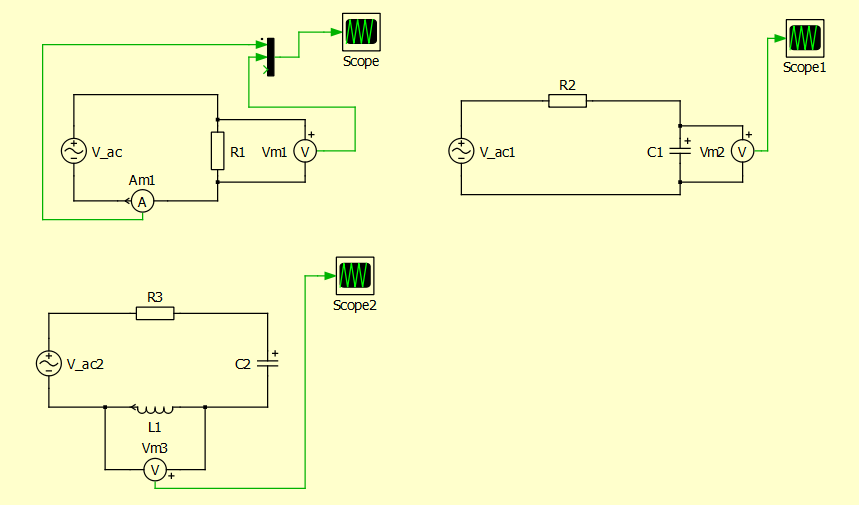
\includegraphics[width=1\textwidth]{Vildledning/Schematics/Eks1_LCR.png}
	\caption{LCR-Kredsløb}
	\label{forslag1}
\end{figure}

Hvor:
\begin{table}[H]
	\begin{tabular}{l|l}
	$R$     & Resistans [\si \ohm] \\
	$V_{ac}$ 	   &  Generator[\si Volt] \\
	$A$ 	   & Ampere-meter [\si Ampere] \\
	$V$			& Volt-meter [\si Volt]
	\end{tabular}
\end{table}
